\documentclass[12pt]{article}

%% FONTS
%% To get the default sans serif font in latex, uncomment following line:
 \renewcommand*\familydefault{\sfdefault}
%%
%% to get Arial font as the sans serif font, uncomment following line:
%% \renewcommand{\sfdefault}{phv} % phv is the Arial font
%%
%% to get Helvetica font as the sans serif font, uncomment following line:
% \usepackage{helvet}
\usepackage[small,bf,up]{caption}
\renewcommand{\captionfont}{\footnotesize}
\usepackage[left=1in,right=1in,top=1in,bottom=1in]{geometry}
\usepackage{graphics,epsfig,graphicx,float,subfigure,color}
\usepackage{amsmath,amssymb,amsbsy,amsfonts,amsthm}
\usepackage{url}
\usepackage{boxedminipage}
\usepackage[sf,bf,tiny]{titlesec}
 \usepackage[plainpages=false, colorlinks=true,
   citecolor=blue, filecolor=blue, linkcolor=blue,
   urlcolor=blue]{hyperref}
\usepackage{enumitem}
\usepackage{verbatim}
\usepackage{tikz,pgfplots}

\newcommand{\todo}[1]{\textcolor{red}{#1}}
% see documentation for titlesec package
% \titleformat{\section}{\large \sffamily \bfseries}
\titlelabel{\thetitle.\,\,\,}

\newcommand{\bs}{\boldsymbol}
\newcommand{\alert}[1]{\textcolor{red}{#1}}
\setlength{\emergencystretch}{20pt}

\begin{document}

\begin{center}
  \vspace*{-2cm}
{\small MATH-GA 2012.001 and CSCI-GA 2945.001, Georg Stadler \&
  Dhairya Malhotra (NYU Courant)}
\end{center}
\vspace*{.5cm}
\begin{center}
\large \textbf{%%
Spring 2019: Advanced Topics in Numerical Analysis: \\
High Performance Computing \\
Assignment 6 (due May 13, 2019) \\ }
Chen Li cl3898@nyu.edu
\end{center}

\noindent {\bf Handing in your homework:} Hand in your homework as for
the previous homework assignments (git repo with Makefile), answering
the questions by adding a text or a \LaTeX\ file to your repo. Some
useful material for this assignment can be found in the repo \url{https://github.com/NYU-HPC19/homework6}.
\\[.2ex]

% ****************************
\begin{enumerate}
% --------------------------
\setcounter{enumi}{-1}

  
\item {\bf Final project update.} Give us an update on the status of
  your final project. You can either just write a paragraph or use a
  table similar as in the previous homework assignment. Keep in mind that
  by the time this homework assignment is due, a big part of the work on the final
  project should be done.
  
  \begin{center}
  \begin{tabular} {|c|p{9cm}|p{2cm}|}
    \hline
    \multicolumn{3}{|c|}{\bf Project: Image Denoising with Total Variation in GPU} \\
    \hline
    Week & Work & Who  \\ \hline \hline
    04/20-04/25 & Read potential paper and algorithm & Chen, Shengqi \\ \hline
    04/26-05/02 & Write pseudo code for the corresponding algorithm  & Chen, Shengqi \\ \hline
    05/02-05/05 &  Implement basic code in C & Chen, Shengqi\\ \hline
    05/06-05/15 & Covert the code into GPU version and debugging & Richard, Erlich \\ \hline
    05/16-05/19 & Run some test for the codes  & Chen, Shengqi \\ \hline
  \end{tabular}
  \end{center}

\item {\bf MPI-parallel two-dimensional Jacobi smoother.} We implement
  a distributed memory (i.e., MPI) parallel version of the
  two-dimensional Jacobi smoother from the second assignment. This is
  an extension of the one-dimensional case available in the class
  repository.\footnote{\url{https://github.com/NYU-HPC19/lecture12.git}}
  We will use a uniform domain splitting as sketched in
  Figure~\ref{fig} and exchange unknowns corresponding to neighboring
  points (the so-called ghost points) on different processors. To make our lives easier, we only
  consider uniform splittings of all unknowns using $p=4^j$,
  $j=0,1,2,3,\ldots$ processors. Additionally we assume that we deal
  with $N=2^jN_l$ unknowns in the $x$ and $y$ directions, such that
  each processor works on $N_l^2$ unknowns.
  \begin{figure}[bht]\centering
  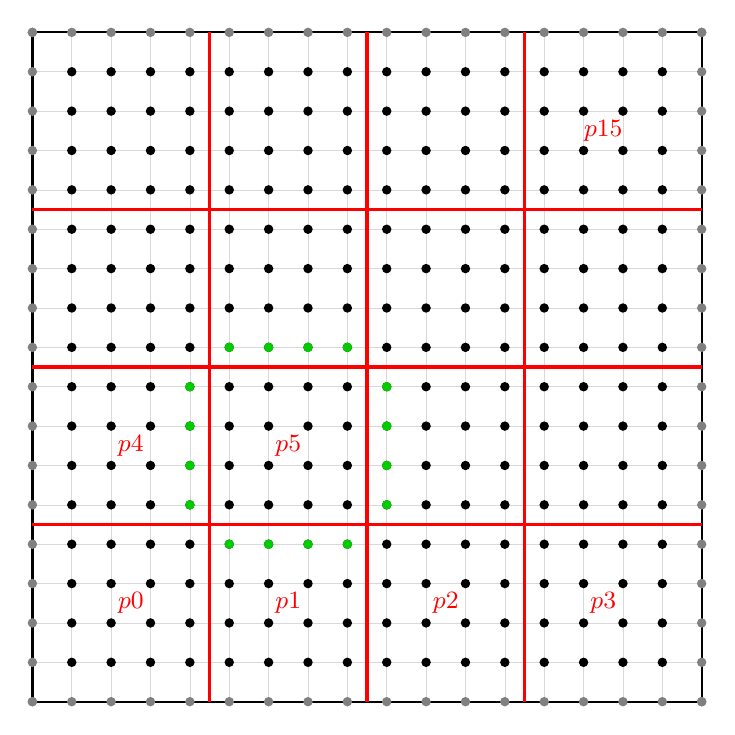
\begin{tikzpicture}[scale=0.5]
    \draw[step=1cm, gray!30!white, very thin] (0,0) grid (17,17);
    \draw[thick] (-0,0) -- (17,0);
    \draw[thick] (0,0) -- (0,17);
    \draw[thick] (0,17) -- (17,17);
    \draw[thick] (17,0) -- (17,17);
    % inner points
    \foreach \x in {1,...,16}
    \foreach \y in {1,...,16}
    \fill[black] (\x,\y) circle (0.12cm);
    \foreach \x in {0,17}
    \foreach \y in {0,...,17}
    \fill[gray] (\x,\y) circle (0.12cm);
    \foreach \y in {0,17}
    \foreach \x in {0,...,17}
    \fill[gray] (\x,\y) circle (0.12cm);
    % ghost points for p=5
    \foreach \xy in {5,...,8} {
    \fill[green!80!black] (\xy,4) circle (0.12cm);
    \fill[green!80!black] (\xy,9) circle (0.12cm);
    \fill[green!80!black] (4,\xy) circle (0.12cm);
    \fill[green!80!black] (9,\xy) circle (0.12cm);
    }
    \foreach \xl in {4.5,8.5,12.5}
    \draw[-,very thick,red] (\xl,0) -> (\xl,17.);
    \foreach \xl in {4.5,8.5,12.5}
    \draw[-,very thick,red] (0,\xl) -> (17,\xl);
    \node at (2.5,2.5) {\small\textcolor{red}{$p0$}};
    \node at (6.5,2.5) {\small\textcolor{red}{$p1$}};
    \node at (10.5,2.5) {\small\textcolor{red}{$p2$}};
    \node at (14.5,2.5) {\small\textcolor{red}{$p3$}};
    \node at (2.5,6.5) {\small\textcolor{red}{$p4$}};
    \node at (6.5,6.5) {\small\textcolor{red}{$p5$}};
    \node at (14.5,14.5) {\small\textcolor{red}{$p15$}};
\end{tikzpicture} \hspace{5ex}
\caption{Uniform splitting of unknowns for parallel computation with
  16 MPI processes, and with $N_l=4$. Unknowns are shown as black
  dots, gray dots are domain boundary unknowns. As example, the ghost
  nodes processor $p5$ requires for updating its values in a Jacobi
  step are shown in green. $p5$ needs to obtain these values through
  communication with $p1,p4,p6,p9$, where they are
  updated.\label{fig}}
\end{figure}
  Before you start coding, figure out a few things:
  \begin{itemize}
    \item For any $p$, find which points (and thus unknowns) must be
      updated by which MPI tasks.
    \item Find which points must be communicated (i.e., the ghost nodes), and between which
      processors this communication must take place.
    \item I suggest following our one dimensional example with blocking
      sends and receives by allocating $(N_l+2)^2$ unknowns for each
      MPI task. The ``inner'' $N_l^2$ points are processed by each MPI
      tasks, while the outer points are used to store and update the
      ghost point copies from neighboring MPI tasks.
  \end{itemize}
Run your implementation on Prince. For large $N_l$ (e.g.,
$N_l=100$), perform a weak scaling study and plot the timings (fix the
number of iterations for this study) as you increase the number of
points and MPI tasks. Then choose $N_l$ as large as possible to fit on
one processor, and perform a strong scaling study, i.e., keep the
problem size unchanged while increasing the number of MPI task, and
plot the speedup compared to the ideal speedup.\\ {\bf Voluntary bonus
  question:} Compare a blocking with a non-blocking implementation, in
which you overlap computation and computation, and study if you
observe a comparison in the run time.\footnote{%
  Recall that the arithmetic intensity of this Jacobi smoother is low
  and thus the problem is memory-bound.}
  
  \textbf{Solution}
  
  Please see code file \texttt{jacobi-mpi-2d.cpp}


\item {\bf Parallel sample sort.}  Each of $P$ processors creates
  an $N$-vector of random numbers. The target is to sort the union of
  all these distributed vectors; this union, let's call it $\bs v$,
  consists of $PN$ numbers and is assumed to be too large to fit into
  the memory of a single processor---thus, a serial sort algorithm
  cannot be used.  The goal is to sort $\bs v$ such that every
  processor roughly holds about $N$ sorted numbers, say $\bs v_i$, and
  that all elements on the processor with rank $i$ are smaller
  than those on the processor with rank $i+1$ (for all $i=0,1,\ldots,
  P-2$).  The above repository contains a stub called
  \texttt{ssort.cpp}. This file also contains an outline of the
  algorithm, which we also discussed in class. For a summary of the
  sample sort algorithm, see the Wikipedia
  entry\footnote{\url{http://en.wikipedia.org/wiki/Samplesort}} for
  sample sort, as well as the pages linked under ``References'' from
  there. The main steps of sample sort are:
\begin{itemize}
\item \emph{Select local samples:} Each of the $P$ processors sorts
  the local array and selects
  a set of $S$ entries\footnote{Choosing $S:=P-1$, as we've used in
    class, is a reasonable choice.} uniformly and communicates these entries to the
  root processor, who sorts the resulting $SP$ entries and determines
  $P-1$ splitters $\{S_1,\ldots,S_{P-1}\}$, which it broadcasts to all
  other processors.\footnote{Note that this step of determining the
    splitters is not necessary if one knows the statistical distribution of the
    random numbers. If that is not known, or each processor holds
    numbers that are distributed very differently, then this step is
    important to find reasonable bins.} 
\item \emph{Distribute to buckets:} Each processor determines the
  ``buckets'' to which each of its $N$ elements belong; for instance,
  the first bucket contains all the numbers $\le S_1$, the second one
  are all the entries that are in $(S_1,S_2]$ and so on. The numbers
    contained in each bucket are then communicated; processor 0
    receives every processor's first bucket, processor 1 gets
    processor's second bucket, and so on.
\item \emph{Local sort:} Each processor uses a local sort and writes
  the result to disc.
\end{itemize}
 Include the MPI rank in the filename (see the example
 \texttt{file-io.cpp} example file).  Run your implementation of
 the sorting algorithm on at least 64 cores of Prince, and present
 timings (not including the time to initialize the input array or the
 time to write output to file) depending on the number of elements $N$
 to be sorted per processor (report results for $N=10^4, 10^5$, and $10^6$).
 
  \textbf{Solution}
  
  Please see code file \texttt{ssort.cpp}

  

\item {\bf Extra credit: Generalize the Multigrid Implementation.} Generalize the
  one-dimensional serial multigrid
  implementation\footnote{To be posted at \url{https://github.com/NYU-HPC19/lecture13}.}
  in at least one (you choose!) of the following directions:
  \begin{enumerate}
    \item Generalize to the two-dimensional problem. From previous
      homework, you already have implementation of the two-dimensional
      Jacobi method. Note that for Jacobi within multigrid, one should
      use a relaxation parameter $\omega$ in the Jacobi update
      step---see the one-dimensional version.
    \item Extend either the one- or the two-dimensional version to a
      shared memory (OpenMP) parallel implementation and run a series
      of large problems on Prince. Report scalability results.
    \item Same but for distributed memory (MPI) version.
  \end{enumerate}


\end{enumerate}
\end{document}
